\subsection{Comparison with other works}

Using the same file types of other works, the ``CLD'' model achieved an accuracy of 
67\% for the file types from Chen \textit{et al.} \cite{chen_file_2018},
91\% for Hiester \cite{hiester_file_2018}, 
59\% for Wang \textit{et al.} \cite{wang_sparse_2018},
65\% for Wang \textit{et al.} \cite{wang_file_2018},
and
61\% for Vulinović \textit{et al.} \cite{vulinovic_neural_2019}.

The accuracy obtained for the dataset including 28 file types was 63\%.

The results can be seen in Figure \ref{fig:cldothers}, in which the bar plot shows the comparison between the validation accuracy obtained with ``CLD'' and those achieved in other studies.

\noindent
\begin{figure*}[htb!]
\centering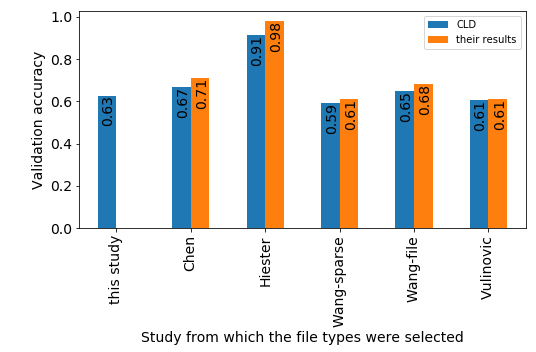
\includegraphics[width=0.8\textwidth]{CLD-others.png}
\caption[CLD vs. other studies]{\label{fig:cldothers}The ``CLD'' model was trained from scratch using the same file types used in other works. The bar plot shows the comparison between the validation accuracy obtained with ``CLD'' and those achieved in other studies. It is interesting to note that changing the dataset file type composition allowed the ``CLD'' model to achieve results similar to those of other works, despite their broad range of values. This suggests that file type composition had a bigger role than model architecture in these results.}%
\end{figure*}

\subsection{Accuracy of pairs of classes}

The data obtained comparing each pair of file types is shown in Table \ref{tab:pcadata}. The comparison of each file type with itself was not performed, but for consistency it was manually filled in the table with the value 0.5.

Figure \ref{fig:dual} shows the graph of the accuracy of each class when compared individually with each one of the others, resulting in 378 models, one for each possible pair of classes. File types where all the points are close to 100\% are hardly mistaken for other types, while accuracy values close to 50\% are the worse results possible, as they are close to random chance.

The results were organized in descending order, using the minimum accuracy result for each file type: pps, ppt, gz, png, dwf, swf, pptx, kmz, jpg, pdf, eps, ps, f, txt, gif, html, xml, doc, xls, sql, hlp, log, kml, java, csv, wp, rtf, dbase3.

\noindent
\begin{figure*}[htb!]
\centering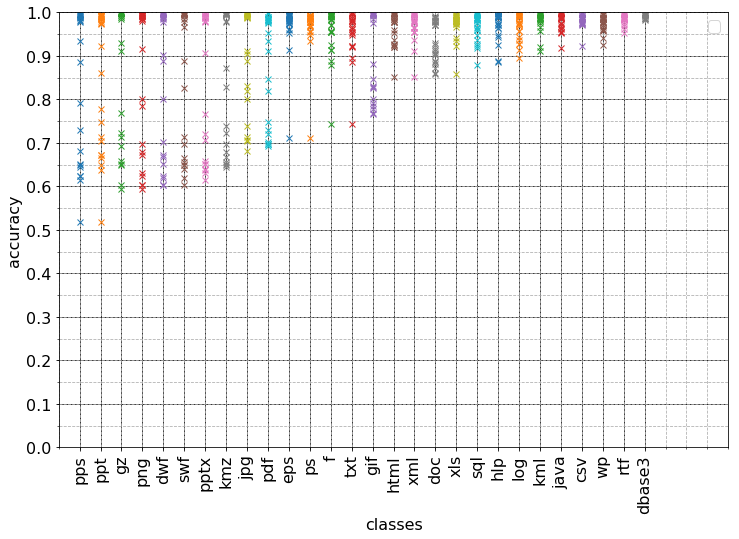
\includegraphics[width=0.8\textwidth]{dual.png}
\caption{\label{fig:dual}Validation accuracy of models trained with pair of classes. File types on the left are assumed to be harder to classify than file types on the right. Later, in the third experiment, this order will be used to select which file types will compose the dataset.}%
\end{figure*}

\begin{table}[!ht]
    \centering
    \caption[Data obtained comparing each pair of file types]{Data obtained comparing each pair of file types}
    \label{tab:pcadata}
                \rotatebox{90}{
    \renewcommand{\arraystretch}{0.8}
    \footnotesize
    \setlength\tabcolsep{1.5pt}
    \begin{tabular}{|l|l|l|l|l|l|l|l|l|l|l|l|l|l|l|l|l|l|l|l|l|l|l|l|l|l|l|l|l|}
    \hline
           & csv  & dbase3 & doc  & dwf  & eps  & f    & gif  & gz   & hlp  & html & java & jpg  & kml  & kmz  & log  & pdf  & png  & pps  & ppt  & pptx & ps   & rtf  & sql  & swf  & txt  & wp   & xls  & xml  \\ \hline
    csv    & 0.50 & 1.00   & 0.99 & 1.00 & 0.98 & 0.97 & 1.00 & 1.00 & 0.98 & 0.98 & 0.97 & 1.00 & 0.98 & 1.00 & 0.97 & 1.00 & 1.00 & 1.00 & 1.00 & 1.00 & 0.99 & 0.99 & 0.98 & 1.00 & 0.92 & 0.99 & 0.99 & 0.98 \\ \hline
    dbase3 & 1.00 & 0.50   & 0.99 & 1.00 & 1.00 & 1.00 & 1.00 & 1.00 & 0.99 & 0.99 & 0.99 & 1.00 & 0.99 & 1.00 & 1.00 & 1.00 & 1.00 & 1.00 & 0.99 & 1.00 & 0.99 & 1.00 & 0.98 & 1.00 & 1.00 & 1.00 & 0.99 & 1.00 \\ \hline
    doc    & 0.99 & 0.99   & 0.50 & 0.90 & 0.98 & 0.97 & 0.88 & 0.93 & 0.97 & 0.98 & 0.99 & 0.90 & 0.98 & 0.87 & 0.99 & 0.91 & 0.92 & 0.89 & 0.86 & 0.91 & 0.97 & 0.99 & 0.98 & 0.89 & 0.98 & 0.93 & 0.86 & 0.98 \\ \hline
    dwf    & 1.00 & 1.00   & 0.90 & 0.50 & 1.00 & 0.99 & 0.80 & 0.60 & 1.00 & 1.00 & 1.00 & 0.89 & 1.00 & 0.67 & 0.99 & 0.70 & 0.60 & 0.62 & 0.67 & 0.65 & 0.98 & 1.00 & 0.99 & 0.62 & 1.00 & 0.99 & 0.98 & 1.00 \\ \hline
    eps    & 0.98 & 1.00   & 0.98 & 1.00 & 0.50 & 0.91 & 1.00 & 0.99 & 0.99 & 0.98 & 0.99 & 0.99 & 1.00 & 0.99 & 0.98 & 0.95 & 0.99 & 0.98 & 0.97 & 0.99 & 0.71 & 0.96 & 0.96 & 0.99 & 0.98 & 0.99 & 0.98 & 0.98 \\ \hline
    f      & 0.97 & 1.00   & 0.97 & 0.99 & 0.91 & 0.50 & 1.00 & 1.00 & 0.89 & 0.93 & 0.95 & 0.99 & 0.99 & 0.99 & 0.91 & 0.99 & 0.99 & 1.00 & 0.99 & 0.99 & 0.96 & 0.99 & 0.88 & 1.00 & 0.74 & 0.96 & 0.98 & 0.95 \\ \hline
    gif    & 1.00 & 1.00   & 0.88 & 0.80 & 1.00 & 1.00 & 0.50 & 0.77 & 1.00 & 1.00 & 1.00 & 0.83 & 1.00 & 0.83 & 0.99 & 0.85 & 0.78 & 0.79 & 0.78 & 0.77 & 0.99 & 1.00 & 0.99 & 0.83 & 1.00 & 0.98 & 0.97 & 1.00 \\ \hline
    gz     & 1.00 & 1.00   & 0.93 & 0.60 & 0.99 & 1.00 & 0.77 & 0.50 & 1.00 & 1.00 & 1.00 & 0.91 & 1.00 & 0.72 & 1.00 & 0.69 & 0.59 & 0.65 & 0.71 & 0.66 & 0.98 & 0.99 & 1.00 & 0.65 & 1.00 & 0.99 & 0.99 & 1.00 \\ \hline
    hlp    & 0.98 & 0.99   & 0.97 & 1.00 & 0.99 & 0.89 & 1.00 & 1.00 & 0.50 & 0.93 & 0.96 & 0.99 & 0.99 & 1.00 & 0.94 & 1.00 & 0.99 & 0.99 & 0.99 & 0.99 & 0.99 & 0.99 & 0.95 & 1.00 & 0.89 & 0.97 & 0.97 & 0.96 \\ \hline
    html   & 0.98 & 0.99   & 0.98 & 1.00 & 0.98 & 0.93 & 1.00 & 1.00 & 0.93 & 0.50 & 0.95 & 1.00 & 0.92 & 1.00 & 0.93 & 0.99 & 0.99 & 0.99 & 0.99 & 1.00 & 0.98 & 0.98 & 0.94 & 1.00 & 0.92 & 0.96 & 0.98 & 0.85 \\ \hline
    java   & 0.97 & 0.99   & 0.99 & 1.00 & 0.99 & 0.95 & 1.00 & 1.00 & 0.96 & 0.95 & 0.50 & 1.00 & 0.98 & 1.00 & 0.97 & 0.99 & 1.00 & 1.00 & 0.99 & 1.00 & 0.99 & 0.99 & 0.92 & 1.00 & 0.96 & 0.98 & 1.00 & 0.96 \\ \hline
    jpg    & 1.00 & 1.00   & 0.90 & 0.89 & 0.99 & 0.99 & 0.83 & 0.91 & 0.99 & 1.00 & 1.00 & 0.50 & 1.00 & 0.74 & 0.99 & 0.82 & 0.80 & 0.68 & 0.70 & 0.71 & 0.99 & 1.00 & 1.00 & 0.71 & 1.00 & 0.99 & 0.99 & 1.00 \\ \hline
    kml    & 0.98 & 0.99   & 0.98 & 1.00 & 1.00 & 0.99 & 1.00 & 1.00 & 0.99 & 0.92 & 0.98 & 1.00 & 0.50 & 1.00 & 0.96 & 0.98 & 0.99 & 0.99 & 0.99 & 1.00 & 0.99 & 0.99 & 0.99 & 1.00 & 0.97 & 1.00 & 0.99 & 0.91 \\ \hline
    kmz    & 1.00 & 1.00   & 0.87 & 0.67 & 0.99 & 0.99 & 0.83 & 0.72 & 1.00 & 1.00 & 1.00 & 0.74 & 1.00 & 0.50 & 0.99 & 0.70 & 0.68 & 0.64 & 0.65 & 0.65 & 0.98 & 1.00 & 1.00 & 0.66 & 1.00 & 0.99 & 0.98 & 1.00 \\ \hline
    log    & 0.97 & 1.00   & 0.99 & 0.99 & 0.98 & 0.91 & 0.99 & 1.00 & 0.94 & 0.93 & 0.97 & 0.99 & 0.96 & 0.99 & 0.50 & 0.98 & 1.00 & 0.99 & 1.00 & 0.99 & 0.96 & 0.97 & 0.93 & 1.00 & 0.89 & 0.98 & 0.97 & 0.94 \\ \hline
    pdf    & 1.00 & 1.00   & 0.91 & 0.70 & 0.95 & 0.99 & 0.85 & 0.69 & 1.00 & 0.99 & 0.99 & 0.82 & 0.98 & 0.70 & 0.98 & 0.50 & 0.70 & 0.73 & 0.75 & 0.72 & 0.93 & 0.99 & 0.98 & 0.70 & 0.98 & 0.98 & 0.98 & 0.98 \\ \hline
    png    & 1.00 & 1.00   & 0.92 & 0.60 & 0.99 & 0.99 & 0.78 & 0.59 & 0.99 & 0.99 & 1.00 & 0.80 & 0.99 & 0.68 & 1.00 & 0.70 & 0.50 & 0.62 & 0.67 & 0.63 & 0.98 & 1.00 & 0.99 & 0.60 & 0.99 & 0.98 & 0.98 & 1.00 \\ \hline
    pps    & 1.00 & 1.00   & 0.89 & 0.62 & 0.98 & 1.00 & 0.79 & 0.65 & 0.99 & 0.99 & 1.00 & 0.68 & 0.99 & 0.64 & 0.99 & 0.73 & 0.62 & 0.50 & 0.52 & 0.61 & 0.98 & 0.99 & 0.99 & 0.65 & 1.00 & 0.98 & 0.93 & 1.00 \\ \hline
    ppt    & 1.00 & 0.99   & 0.86 & 0.67 & 0.97 & 0.99 & 0.78 & 0.71 & 0.99 & 0.99 & 0.99 & 0.70 & 0.99 & 0.65 & 1.00 & 0.75 & 0.67 & 0.52 & 0.50 & 0.64 & 0.99 & 0.98 & 0.97 & 0.66 & 0.98 & 0.97 & 0.92 & 0.99 \\ \hline
    pptx   & 1.00 & 1.00   & 0.91 & 0.65 & 0.99 & 0.99 & 0.77 & 0.66 & 0.99 & 1.00 & 1.00 & 0.71 & 1.00 & 0.65 & 0.99 & 0.72 & 0.63 & 0.61 & 0.64 & 0.50 & 0.99 & 1.00 & 0.99 & 0.64 & 0.98 & 0.98 & 0.98 & 0.99 \\ \hline
    ps     & 0.99 & 0.99   & 0.97 & 0.98 & 0.71 & 0.96 & 0.99 & 0.98 & 0.99 & 0.98 & 0.99 & 0.99 & 0.99 & 0.98 & 0.96 & 0.93 & 0.98 & 0.98 & 0.99 & 0.99 & 0.50 & 0.97 & 0.97 & 0.98 & 0.95 & 0.98 & 0.99 & 0.99 \\ \hline
    rtf    & 0.99 & 1.00   & 0.99 & 1.00 & 0.96 & 0.99 & 1.00 & 0.99 & 0.99 & 0.98 & 0.99 & 1.00 & 0.99 & 1.00 & 0.97 & 0.99 & 1.00 & 0.99 & 0.98 & 1.00 & 0.97 & 0.50 & 0.98 & 1.00 & 0.95 & 0.98 & 0.99 & 0.98 \\ \hline
    sql    & 0.98 & 0.98   & 0.98 & 0.99 & 0.96 & 0.88 & 0.99 & 1.00 & 0.95 & 0.94 & 0.92 & 1.00 & 0.99 & 1.00 & 0.93 & 0.98 & 0.99 & 0.99 & 0.97 & 0.99 & 0.97 & 0.98 & 0.50 & 1.00 & 0.92 & 0.96 & 0.99 & 0.96 \\ \hline
    swf    & 1.00 & 1.00   & 0.89 & 0.62 & 0.99 & 1.00 & 0.83 & 0.65 & 1.00 & 1.00 & 1.00 & 0.71 & 1.00 & 0.66 & 1.00 & 0.70 & 0.60 & 0.65 & 0.66 & 0.64 & 0.98 & 1.00 & 1.00 & 0.50 & 0.99 & 0.99 & 0.97 & 1.00 \\ \hline
    txt    & 0.92 & 1.00   & 0.98 & 1.00 & 0.98 & 0.74 & 1.00 & 1.00 & 0.89 & 0.92 & 0.96 & 1.00 & 0.97 & 1.00 & 0.89 & 0.98 & 0.99 & 1.00 & 0.98 & 0.98 & 0.95 & 0.95 & 0.92 & 0.99 & 0.50 & 0.96 & 0.98 & 0.96 \\ \hline
    wp     & 0.99 & 1.00   & 0.93 & 0.99 & 0.99 & 0.96 & 0.98 & 0.99 & 0.97 & 0.96 & 0.98 & 0.99 & 1.00 & 0.99 & 0.98 & 0.98 & 0.98 & 0.98 & 0.97 & 0.98 & 0.98 & 0.98 & 0.96 & 0.99 & 0.96 & 0.50 & 0.94 & 0.97 \\ \hline
    xls    & 0.99 & 0.99   & 0.86 & 0.98 & 0.98 & 0.98 & 0.97 & 0.99 & 0.97 & 0.98 & 1.00 & 0.99 & 0.99 & 0.98 & 0.97 & 0.98 & 0.98 & 0.93 & 0.92 & 0.98 & 0.99 & 0.99 & 0.99 & 0.97 & 0.98 & 0.94 & 0.50 & 0.98 \\ \hline
    xml    & 0.98 & 1.00   & 0.98 & 1.00 & 0.98 & 0.95 & 1.00 & 1.00 & 0.96 & 0.85 & 0.96 & 1.00 & 0.91 & 1.00 & 0.94 & 0.98 & 1.00 & 1.00 & 0.99 & 0.99 & 0.99 & 0.98 & 0.96 & 1.00 & 0.96 & 0.97 & 0.98 & 0.50 \\ \hline
    \end{tabular}
    }
\end{table}


\subsection{Accuracy vs. number of classes}

% decrease in accuracy
The results of the accuracy versus number of classes experiment are shown in Figure \ref{fig:nclasses}.  Each point in the graph is the validation accuracy of a distinct model trained with the indicated number of classes. The class for a block sample is the file extension of the original file. 

The ``models trained with many classes'' are the 135 results obtained by using a random selection of file types to compose the dataset.

The ``models trained with 2 classes'' are the 378 results obtained in the previous experiment, using transparency to improve visualization, as many of them are too close. 

The smooth ``random chance''line in the bottom indicates for comparison how accurate a random guess classifier would be.

% For 2 classes, the accuracy values are between 50\% and 100\%, with a greater concentration near 100\%. For 28 classes, the accuracy values are between 55\% and 58\%.

The lines ``hard file types first'' and ``easy file types first'' were created by selecting the file types that would compose the dataset. The selection was based on the results described in the previous experiment, ``Accuracy of pairs of classes'', ordering the file types by their minimum accuracy values and following this order to choose file types. For example, the ``hard file types first'' point for three classes was obtained by training a model with the file types ``pps'', ``ppt'', and ``gz'', the three classes with lower minima in Figure \ref{fig:dual}.

\noindent
\begin{figure*}[htb!]
\centering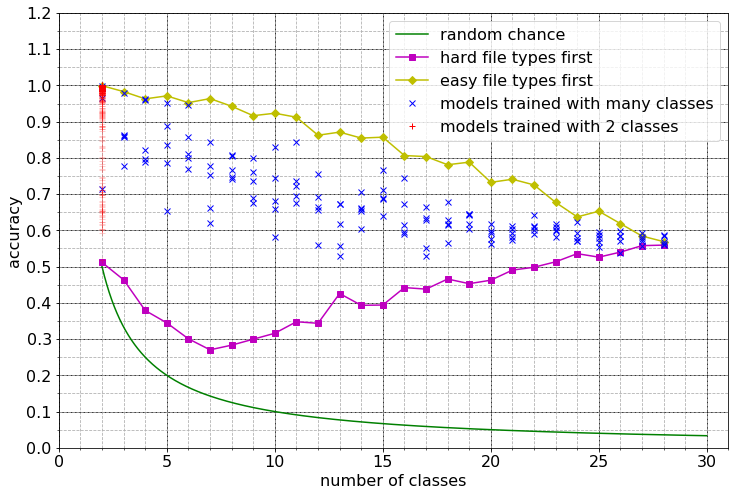
\includegraphics[width=0.8\textwidth]{nclasses.png}
\caption{\label{fig:nclasses}Validation accuracy by number of classes. This graph shows how the choice of the file types composing the dataset influences the validation accuracy of the model. A random choice of file types (the ``models trained with many classes'' line) may seem to yield an accuracy that decreases linearly with the number of classes. But this would be an incomplete conclusion, as not all file types have the same impact on accuracy. This is shown in the lines 
``hard file types first'' and ``easy file types first''. Using a carefully chosen set of file types, is possible to raise or decrease the model accuracy. For example, a model trained with the 15 file types that were considered harder had an accuracy of 39\%, while  a similar model trained with the 15 file types considered easiest had an accuracy of 85\%.}%
\end{figure*}

